\setcounter{figure}{0}
\renewcommand{\thefigure}{4-\arabic{figure}}

\section[第四章\q 技术分析]{第四章\\ 技术分析}

\subsection{技术分析的基石}

{\kaishu
技术分析者不问为什么。那么问为什么的人，就不是技术分析者。

\hfill ——金融帝国
}

技术分析是从市场的真实走势入手，对未来的走势进行一定程度的研判。如果说，价格是由众多原因影响后形成的结果，那么基本分析就是用现在的原因，推导未来的原因，从而再推导出未来的结果；而技术分析则是用现在的结果推导未来的结果。似乎，技术分析来得更直接一些。下面，我们先来看看技术分析的三大假设。

第一，市场行为涵盖一切信息。确切地说，这个假设是不完全正确的。按照“冰山原理”的说法，能够影响市场的信息是无限的，那么无限的信息又如何被唯一并且真实的价格所包容呢？被市场考虑到的信息是有限的，而未被市场考虑到的信息是无限的。那么应该是，市场行为涵盖了被全部交易者考虑到的一切信息。按照“巨变效应”的说法，信息是可以被封存起来的。也就是说，一则消息可能当时并没有被市场全部反映，而是被市场封存起来。当达到临界状态后，这种被封存的因素又会随时被快速释放出来。

当我在思考看外盘是否对第二天的交易有意义的时候，得出这样一个结论：如果外盘与国内具有100％相关性的话，那么看外盘只不过是提前知晓第二天出现的盈亏，而对实盘操作没有丝毫的意义。但如果外盘与国内走势毫无相关性的话，那么看外盘连提前知晓第二天的开盘走势都不可能，并且同样对实盘操作没有丝毫意义。由此可知，无论外盘与国内具有多大的相关性，通过外盘的提示作用而获取利润都是不可能的。这不难理解，外盘的影响都能被市场迅速包容，而无论这种影响具体有多大。这时市场既是接收信息反映的运动员，又是决定如何反映的裁判员。如果把“外盘”理解成信息的话，那么就能得到这样的结论：市场行为涵盖一切它应该涵盖的信息。也就是说，能够涵盖信息的已经涵盖了，而没有涵盖的又是市场裁定为与市场无关的信息。信息与市场是否有关、或者关系多大，完全由市场说了算。这样一来，这种似乎有点废话般的逻辑变得无懈可击了。

至于被封存起来的信息，市场只是暂时裁定并且消化了它的价值。问题在于，封存起来的信息何时、会以什么方式释放出来，对于我们来说是完全不可知的。就好像即使我们能够知晓地震发生的机制，也仍旧无法准确地预测地震会在何时、何地发生一样。对于临界状态的不可知性，大家可以看看《临界》这本书。那么，技术分析的第一假设应该为：走势说明一切。我们不在这里咬文嚼字了，技术分析第一大假设的意义在于：任何公开消息都不具有超越市场本身的价值。

第二，价格呈趋势运行。这一点应该是毫无疑问的。过去两年上证指数从998点上涨至6124点，这种现象很难用漫步随机来解释。如果真的是每天抛一次硬币，然后根据正反面来绘制一种图形的话，那么可能一万年也无法绘制出类似股市走势的图形来。期货市场存在的价值就在于为套期保值者提供场所。如果商品价格不存在大幅度的趋势波动，那么期货市场就失去了存在的意义。无论从任何角度来看，价格呈趋势运行都是无懈可击的。

第三，历史会重演。世界上没有两片树叶是相同的，所以历史和未来也不会绝对相同。但是人性是相同的，并且又是很难改变的。如果说市场是人性的一面镜子的话，那么历史与未来会有某些趋同性，就丝毫不会让人感到奇怪了。无论是荷兰郁金香狂潮，还是英国南海泡沫，或者是美国佛罗里达泡沫，我们都能从中看到人性的轨迹。已有的事，后必再有；已行的事，后必再行。日光之下，并无新事。也许事物的表面在不断变化，但事物的本质通常是很难改变的。

在我看来，技术分析的精髓在于，只考虑市场是什么，而跳过市场为什么是什么。所以，技术分析不问为什么。通常来说，寻找规律要比弄清机制（成因）简单得多。上个世纪三大理论发现之一的量子理论除了它的精确以外，科学家对它一无所知。或者说，科学家只知道量子理论是什么，但至今没有人知道量子理论为什么会是这样？技术分析有点类似于量子理论，它寻找规律、研究现象，而对形成规律、现象的原因并不感兴趣。

正统的技术分析，属于统计学的范畴。它只能得出未来的概率分布，而不可能得出未来一定会出现的结果。这种基于概率的分析方法，就注定了“多次有效、单次无效”的特征。或者说，技术分析能够用于交易获利，但无法用于行情预测。

在我看来，技术分析最大的优势在于，它是一种平民化的获利武器。它唯一的进入门槛就是从网上下载一个行情软件，而无需更多的其他支出。在数据传输技术非常发达的21世纪，技术分析的成本几乎可以降低到忽略不计的程度。上个世纪90年代，我为了使用技术分析，不得不花费近万元来购置电脑与分析软件，并且每年还要花费近千元的数据传输费用。要知道那时我控制的资金量还不到六位数。

按照“巨变效应”“恐龙效应”“钟摆效应”，我们可以得知所谓的规律分为宏观规律和微观规律。这就引申出一个问题，规律来源于重复，而重复又有可能意味着改变。那么在技术分析中应该如何应对这些问题呢？这些相对复杂的问题我们稍后再加以讨论，而本章着重讨论技术分析方法的单个板块。他们分为：技术指标、形态分析、K线分析、切线理论、波浪理论、江恩理论。

\subsection{技术指标}

技术指标是对历史数据，通过一定的公式而计算得出的指标。虽然技术指标的种类很多，但基本上可以分为三类，那就是“趋向指标”“摆动指标”“综合指标”。

首先，对于趋向指标而言，它们的核心思想就是捕捉趋势，一定幅度的上涨就是买入的理由，一定幅度的下跌就是卖出的理由。而不同的趋向指标之间的区别，则完全体现在如何对“一定幅度”进行定义。基本上来说，它们的始祖就是移动平均线。后期又逐步发展出加权移动平均线（EX-PMA）、平滑异同移动平均线（MACD）、抛物线指标（SAR）等。其实，某软件中“S点买入，B点卖出”的指标也属于趋向指标。甚至从广义上来讲，“哈奇10％投资法则”也属于趋向指标的范畴。这些趋向指标，虽然种类繁多，但基本上大同小异。如果你研究它们的计算公式的话，你会发现它们的原理都是极其简单的。

正统的趋向指标，就是一个趋势跟踪系统。它们不会因为涨得高而卖出，也不会因为跌得多而买入。在我看来，这种没有思维的跟踪策略，往往好于99％的交易者作出的分析。我相信，对于某些特定的微观行情而言，不同参数的趋向指标可能会产生天壤之别的结果。但如果你能够交易足够长的时间，并且从整体的宏观上来考察的话，那么所有趋向指标最终的操作结果应该是趋同的。这说明，没有最好的指标，只有最适合自己的指标。

对于移动平均线而言，有“葛兰碧八大买卖法则”，其中就引申出“乖离率”的思想。其实乖离率应该算是一种“摆动指标”，但同时它又架构在“趋向指标”的基础之上。与此类似的就是布林线（BOLL），它的核心就是一个参数为20的移动平均线，而上下轨也是通过“摆动指标”的思想发展出来的。在我看来，这种“既求势又求价”的思想，几乎没有什么可操作性。简单地说，它们具备了“趋向指标”与“摆动指标”的全部优势，同时也承担了全部的成本。而趋势与整理又是对称的，一种方法的优势就是另外一种方法的成本。趋势跟踪系统讲究用少数的大利润来对冲多次的小亏损，如果我们将少数的大利润也限制其增长，那么最终的结果就只能是失败。

我想谁都无法否认，趋向指标在强劲趋势面前的价值。但更多的人，都是只知道趋向指标能够获利，但却很少有人意识到趋向指标的正确率是低于50％的，甚至无法避免“买在最高点和卖在最低点”的可能。很多“高手”都在想尽一切办法来克服这种趋向指标先天性的缺陷。而我认为，如果你不能接受和包容这种缺陷，那么你就不可能享受趋势跟踪的必然利润。

其次，对于摆动类指标而言。它们的核心思想就是捕捉整理行情，一定幅度（强度）的上涨就是卖出的理由，一定幅度（强度）的下跌就是买入的理由。它们包括：相对强弱指标（RSI）；随机指标（KDJ）；威廉指标（WMS）等。从广义上来看，心理线（PSY）、“支撑／阻力位”等，一切限定涨跌幅度和强度的指标都属于摆动类指标。

摆动指标的波动范围通常在0到100之间，这是由于摆动指标通常以一段时间内上涨（下跌）幅度与整体波动幅度的对比关系决定。这种特性又决定了，当趋势出现后涨跌对指标的影响产生不对称性。比如，RSI越接近100或者0就越困难，而50呈现一种对指标的吸引力。

既然有架构在趋向指标基础之上的摆动指标，那么同样也有架构在摆动指标基础之上的趋向指标。有人曾经以RSI指标钝化作为买卖信号，“超买”不但意味着整理行情会出现回调，更意味着趋势行情有可能开始。这种思维方式后来又演化出顺势指标（CCI），并以指标数值超过正负100作为趋势可能出现的信号。

如果机械按照摆动类指标操作的话，那么正确率应该是高于50％的。大家都知道这种正确率的优势，但很少有人愿意相信按照摆动指标操作会偶尔（但必然会出现）遭受大幅度的亏损。很多“高手”希望通过指标的改良，而规避这种偶尔出现的大幅亏损。但这样一来，又会大幅度地降低该类指标的正确率。道理很简单，这种高正确率正是因为对利润的限制，以及对亏损的“不设防”才能够产生的。

这里我只能说我并不使用、甚至是参考摆动类指标，那么批判自己并不使用的分析方法似乎没有任何意义。我只想提醒大家一点，不要被摆动类指标的“视觉效果”所迷惑。KDJ等指标几乎总是在低位金叉、在高位死叉，似乎我们总是能够通过不断摆动来获利。但请注意，这只不过是指标的高低位，而并不是价格的高低位。如果大家真的希望使用摆动类指标，那么必须要进行充分的测试来验证你所采用的技术具有可行性。我最多只能说，我并不具备使用摆动类指标获利的能力，那么在我眼中这种努力自然是非常困难的。

最后，对于综合类指标而言，它们或是加入成交量的因素，或是采用与其他品种（指数）对比的思路，或是从市场的内部结构特征入手。总之这类指标并不完全以单一品种的价格波动作为全部的考虑因素。

对比思路是一种不错的思维方式。比如，相对强弱指数，它是以个股收盘价除以指数收盘价而绘制成的连续走势图。该指数的具体数值并不重要，重要的是指标走势的发展。如果相对强弱指数不断走强，那么就说明该股在反复相对于大盘走强，从而可以预期该股未来会进一步强于大盘。这种方法是纯技术分析派，选股时的绝佳工具。与此类似的还有，威力雷达等指标。

腾落指标（ADL）是一种测量市场广度的常用指标。当价格上涨的股票数超过价格下跌的股票数时，腾落指标向上移动，这表示股市强劲；反之，则说明股市疲软。它是根据股市内部个股涨跌的分布状况，来研判未来走势的一种方法，对于战略性的宏观分析具有明显的提示作用。在后面的文章中大家会发现，我是非常重视“市场广度”的问题的。

能量潮指标（OBV）是一种成交量累加指标，收出阳线时，将成交量加入OBV指标；收出阴线时，用OBV数值减去当日成交量。由于上涨时成交量通常较下跌时大，所以OBV指标通常为正值，而且上市时间越长的股票，OBV的数值越大。这种技术指标的思想在于，观察价格波动能否得到成交量的配合。对于我的交易习惯来说，我更加注重信号的必然性，而并非信号的准确性。也就是说，我是不会将这类指标作为趋势跟踪的过滤器，而是追求只要有超过一定幅度的趋势行情，我就必然要赚到属于自己的利润。当然换一个角度，将该指标用于从股票池中挑选股票，似乎并没有任何不妥。由此看来，对于一种指标的使用，不可能不考虑交易者自身的整体思路。

综合类指标一般只能当做参考使用，而不能发出绝对的买卖信号，更难以将其加入操作系统中。由此看来，综合指标更容易被运用于分析与预测，而对实战只能起到一些提示作用。

在技术指标的使用过程中，我们经常可以遇到钝化、背离等问题。对于钝化而言，它是指摆动类指标长期处于超买或超卖位置。假设市场处于整理阶段，摆动类指标就不会出现钝化。那么出现钝化时，就提示我们趋势行情有可能产生。对于背离而言，他的原理完全来自于指标0轴、或者中间值具有的“吸引力”，而造成涨跌对于指标数值影响的不对称性。简单地说，就是价格创新高（低），而指标没有创新高（低）。请注意，价格创出新高时，指标都无法立刻创出新高！

这是一个很有趣的错觉：无论真假突破，突破当时指标都是背离的。而没有背离的情况，只不过是因为突破后价格大幅上涨，之后再进行观察的结果。这是明显的未来函数，突破当时我们无法通过“背离”来验证突破的真假，而当突破早已被证实真假以后，再套用“背离”的说法进行“验证”并没有任何意义。只要价格创出新高，而指标没有创出新高，就认为是“背离”而卖出，绝对是大众一种明显的误区。

\subsection{形态分析}

{\kaishu
如果一种分析方法能够将未来所有的可能都囊括其中，并且可以作出合理的解释，那么这种分析方法基本上就没有任何实战价值了。

\hfill ——金融帝国
}

形态分析将走势图中的形态分为“反转突破形态”和“持续整理形态”两种。其中“反转突破形态”包括：双顶（低）、三重顶（低）、头肩顶（低）、圆弧顶（低）、V形反转；而“持续整理形态”包括：矩形、三角形、旗形、楔形。

在我看来，形态分析对于反转形态归纳得比较细致，基本上囊括所有反转时可能出现的情况。但对于整理形态，似乎归纳得并不细致。整理形态本质上是趋势中的一次调整。如果加上“波浪理论”中的调整形态，那么整理形态就基本上完备了。波浪理论中将能够划分为三个子浪的简单调整分为：之字形调整、平坦形调整。而对于复杂的“双3”和“三3”，基本上很少能够在日线以上的级别中出现。有意思的是，波浪理论中也有三角形，这与形态理论别无二致。

在我看来，单独的形态分析的预测意义与可操作性基本上是不存在的！形态分析不过是一种对市场的解释工具，它能够把市场任何可能出现的走势形态都囊括其中。也就是说，无论未来市场如何运行，形态分析都能将其合理地纳入其中。这样一来，形态分析就不能算做什么分析了，而只能算是一种自欺欺人的幻觉追求工具。我想这时大多数人都不能接受我这种偏激的结论，那么就听听我的理由吧！为了阐述的方便，我们全部以上涨行情为例，其实下跌的道理也是完全相同的。

如果上涨中出现一次下跌的话，那么见顶了就是V形反转。而如果其后创出新高就是一次“简单的调整”。当然这种简单调整没有纳入“形态分析”和“波浪理论”当中，但是谁也无法否认市场中经常会出现这种简单、短暂的调整。也许是这两种理论都认为这种情况太普遍而不值得一提吧。

\begin{figure}[H]
\centering
\captionsetup{font=footnotesize}
\begin{minipage}[t]{0.18\linewidth}
\centering
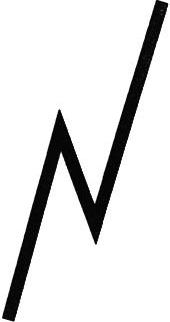
\includegraphics[width=\linewidth]{images/4-1简单调整.jpg}
\captionof{figure}{简单调整}\label{fig:simple-adjustment}
\end{minipage}\hfill
\begin{minipage}[t]{0.18\linewidth}
\centering
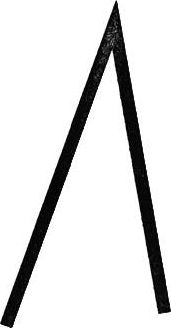
\includegraphics[width=\linewidth]{images/4-2V形反转.jpg}
\captionof{figure}{V形反转}\label{fig:v-reversal}
\end{minipage}\hfill
\begin{minipage}[t]{0.18\linewidth}
\centering

\includegraphics[width=\linewidth]{images/4-3双头.jpg}
\captionof{figure}{双头}\label{fig:double-head}
\end{minipage}\hfill
\begin{minipage}[t]{0.18\linewidth}
\centering
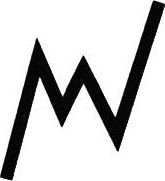
\includegraphics[width=\linewidth]{images/4-4之字形调整.jpg}
\captionof{figure}{之字形调整}\label{fig:zigzag-adjustment}
\end{minipage}\hfill
\begin{minipage}[t]{0.18\linewidth}
\centering
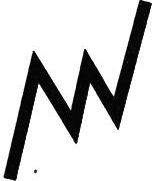
\includegraphics[width=\linewidth]{images/4-5平坦形调整.jpg}
\captionof{figure}{平坦形调整}\label{fig:flat-adjustment}
\end{minipage}\par\medskip
\begin{minipage}[t]{0.18\linewidth}
\centering
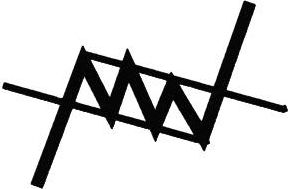
\includegraphics[width=\linewidth]{images/4-6旗形整理.jpg}
\captionof{figure}{旗形整理}\label{fig:flag-consolidation}
\end{minipage}\hfill
\begin{minipage}[t]{0.18\linewidth}
\centering
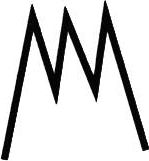
\includegraphics[width=\linewidth]{images/4-7三重顶.jpg}
\captionof{figure}{三重顶}\label{fig:triple-top}
\end{minipage}\hfill
\begin{minipage}[t]{0.18\linewidth}
\centering
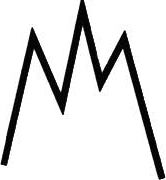
\includegraphics[width=\linewidth]{images/4-8头肩顶.jpg}
\captionof{figure}{头肩顶}\label{fig:head-and-shoulders}
\end{minipage}\hfill
\begin{minipage}[t]{0.18\linewidth}
\centering
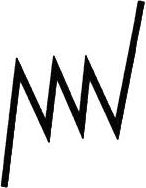
\includegraphics[width=\linewidth]{images/4-9矩形.jpg}
\captionof{figure}{矩形}\label{fig:rectangle}
\end{minipage}\hfill
\begin{minipage}[t]{0.18\linewidth}
\centering
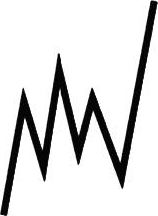
\includegraphics[width=\linewidth]{images/4-10跨过顶部是天空.jpg}
\captionof{figure}{跨过顶部是天空}\label{fig:sky-beyond-top}
\end{minipage}
\end{figure}




那么如果第一次的下跌出现反弹后又继续下跌时，就又出现了三种可能。如果最终见顶，那么就是双顶；如果没能见顶、并且又没有创出第一次的新低，那么就是平坦形调整。如果没能见顶、并且创出了第一次的新低，那么就是之字形调整。请注意，之字形调整与双顶是矛盾的！事实上，之字形调整就是双顶跌破颈线（成立）后，就立刻见底上扬的形态。站在最低点的时点上来看，之字形调整是一个完美的双顶形态。有意思的是，这种形态理论无法解释的现象，却是在市场中经常出现的！我将其称为“假双顶”，并且这种形态不但符合波浪理论，而且还是具有极佳提示作用的形态。这一点，我们在“雕虫小技”中详细探讨。确切地说，还有第四种可能，那就是“旗形”与“楔形”在形成过程中的情况。这两种形态是允许第二个低点低于（第一个低点的水平）颈线的。












那么如果第二次的下跌出现反弹后又继续下跌时，同样出现了三种可能。如果最终见顶，那么就是三重顶或者头肩顶；如果没能见顶的话，那么因当时特点将其归纳为形态理论的“持续整理形态”。要知道无论走势如何，都能将其归纳为矩形、三角形、旗形、楔形等形态中。不信你试试看，五浪的调整，你还能找出这几种可能性之外的画法吗？对于上面提到的旗形和楔形来说，就出现了一种事后合理的幻觉。对于跌破水平颈线后下跌的案例，我们就很自然将其归纳为顶部形态；而对于跌破水平颈线后就立刻见底的部分案例，我们就会同样自然地将其归纳为旗形或者楔形。当然还有一种可能就是跌破头肩顶的颈线后，就立即见底的情况。由于头肩顶中间的顶高于前后两个顶，那么就没有办法将其解释为旗形或者楔形。这时就出现了“假头肩顶”（波浪理论称为“头肩形整理”，我后面称其为“跨过顶部是天空”），后面我会着重解释这种情况。













第三次下跌后出现的上涨，根据江恩的“四次法则”，就此展开升势的概率是极大的。从历史统计中，我们也很难在大尺度上找到更长次数整理的案例。但如果行情真的陷入更复杂的整理中，那么就可以用波浪理论中“双3”和“三3”，以及“九浪三角形”来解释。由此看来，通常的整理都会在三次下跌后结束。这似乎又回到了《狼来了》的故事，以及“事不过三”的老俗话中来。我要说的是，当整理出现之前，你并不知道是横向整理；而当你看出这是整理行情的时候，通常意味着整理行情的结束！

上面阐述的是形态的划分，而形态分析中三大提示，在我看来全部都是误区！首先，调整形态通常都是缩量的。这个命题的正确率几乎接近100％。但如果反过来看，反转形态在形成过程当中也是缩量的！这个命题的正确率同样接近100％！对于上涨行情而言，推动趋势就需要巨大的成交量，而横向运行无论是整理还是反转通常都是缩量的！形态分析对于双顶的描述中，也有“第一次下跌后的上涨，在成交量萎缩的情况下而不能创出新高”的说法。事实上，成交量是与价格同步，而从来没有领先过价格。遗憾的是，很多股民在“调整”（下跌）中，以成交量萎缩作为不卖出的理由。如果调整后又继续上涨，那么就可以将其归纳为整理形态；而与此同时，缩量后又继续放量，仍旧可以归纳为整理形态。但如果“调整后”继续下跌，那么就可以归纳为反转形态；而与此同时，缩量后继续缩量，仍旧可以归纳为反转形态。请注意，他们是同步的，而成交量并没有提示作用。我们从OBV指标也能看出，成交量在上涨的时候通常要比在下跌的时候大，这也是通常OBV指标都是正值的原因。这种现象告诉我们一个非常重要的道理：衡量一个命题好坏的标准，不光是正确率的问题，更重要的是符合这种命题，但不成功的比例具体有多大？比如，人类的生存都是需要呼吸氧气的。这个命题的正确率是100％，但如果根据这个命题作出“呼吸氧气的就是人类”的判断，那么就有点贻笑大方了！

其次，三重顶比头肩顶更容易演化成持续整理形态。形态理论的根据是认为，三重顶有更多类似于矩形整理的特征。但我从更多的历史走势中发现头肩顶跌破颈线“确立”顶部后就立刻大涨的案例。更有意思的是，这类案例后期的上涨不但快速，而且升幅巨大！我将这种头肩顶成立后又演化成整理形态的走势称为“跨过顶部是天空”，并且该形态是最佳的快速获利形态。这种形态理论解释不了的现象，却能够与波浪理论不谋而合！按照波浪理论的说法，三浪上涨与四浪下跌组成了头肩顶的左肩；五浪上涨与A浪下跌组成了头肩顶的头；而B浪反弹与C浪下跌组成了头肩顶的右肩。而这种相对强劲上涨后出现的强势调整，通常为大三浪的第一和第二子浪。后期出现快速而大幅上涨的“三浪三”就不足为奇了。

最后，跌破颈线后的最小跌幅等于最高点与颈线的垂直距离。我个人感觉这种说法是没有任何统计学依据的。通常来说，反转形态如果能够成立的话，那么事后来看，通常下跌都能够大幅度地超过最小跌幅。而如果出现“假双顶”与“跨过顶部是天空”时，下跌的幅度又会小于最小跌幅。要知道这两种情形出现的次数应该大于形态分析中的“反转突破形态”的次数。

道理很简单，调整浪都会是奇数浪。稍加统计，我们都不难发现这样的规律：调整次数越多的整理形态，出现的次数就越少。1浪调整最多，而无论是波浪理论还是形态理论，都将其视为上涨的一部分而不加描述；3浪调整其次，只有波浪理论进行描述，但形态理论却没有任何描述；5浪调整很少出现，也就是说，形态理论中的“持续整理形态”只不过是全部整理形态的一小部分；7浪调整极少出现，波浪理论将其解释为“双3”；再多的调整次数都可以用波浪理论中“九浪三角形”与11浪调整组成的“三3”来解释。我的意思是说，反转形态在趋势中只能出现一次，而由5浪调整形成的形态理论中的“持续整理形态”出现的次数要小于“波浪理论”中“ABC三浪调整”的次数。这样一来，“假双顶”与“跨过顶部是天空”不但不是偶然现象，反而出现次数要大于形态理论中描述的任何形态。

\textbf{由此看来，形态分析只能把已经完成的走势进行归类，而对于未来的走势没有任何提示作用。遗憾的是，这种分析方法被编入《期货从业资格教材》，甚至被大量的交易者使用。}想想也很讽刺，交易者乐意相信未来会如何运行，都可以按照形态理论进行假设。我真想不明白，这个行业内的所有角色、所有参与者，到底还要在事后合理的幻觉中走多远？曾经的我，因为误信形态理论而遭受过惨重的亏损，但由此我也找到了一种高效的获利方法。

\subsection{K线分析}

{\kaishu
请相信我，大家都在谈论的分析方法，并不一定就是对的。

\hfill ——金融帝国
}

K线又称阴阳线、棒线、红黑线或蜡烛线，起原于日本德川幕府时代（1603—1867）的米市交易。起初K线只不过是一种走势记录工具，将复杂的日内波动浓缩为一个有代表性的“符号”。但经过200多年的演进，形成了现在具有完整形式和分析理论的一种技术分析方法。

K线的制作并不复杂，只包含最高价、最低价、开盘价、收盘价，四个重要元素。开盘价高于收盘价为阴线、低于收盘价为阳线。我不得不承认K线是一个伟大的发明，他将复杂的走势归纳为一个非常直观的符号。由此看来，K线是一门忽略的艺术，将大量琐碎的信息进行忽略，而让我们能够一目了然地了解到一段时间内价格波动的大体特征。对于初学者而言，进入市场最先学习的可能就是看K线。十年前由于科技不发达，远没有现在这么方便的数据传输工具。我为了研究K线走势，只好从报纸上收集信息，然后用笔来人工绘制K线。事实上，手工绘制K线确实能够培养一种不错的市场感觉，有时间的交易者不妨试试看。

后人背弃了K线发明者“化繁为简”的初衷，而发明了众多繁琐的K线理论。这里我们不过多介绍这些理论，而是谈谈我对K线理论的看法。

首先，命题的事后正确率并不能代表什么。在上面的“形态分析”中我讲述了，一种结果通常是由一种原因形成的，但不等于这种原因通常会形成这种结果。我们可以从历史走势图中，轻松地找到“射击之星”“乌云盖顶”“穿头破脚”“三只小乌鸦”等一系列的顶部形态。最早我在1997年看青木的《战胜庄家》时，作者指出出现“十字星”通常意味着后期会有不寻常的走势，底部有“吸货十字星”、顶部有“出货十字星”。巧得很，上证指数在1997年5月的顶部正好出现了一个标准的十字星。几年后我发现一个不容忽视的问题：在趋势的运行中同样会出现众多无效的“十字星”，这该如何是好呢？假设，所有行情的顶部都能出现一种信号，“事后正确率”为100％，但在顶部形成之前，同样的信号会出现10次无效的案例。那么这种信号的价值又是什么呢？除非你能通过离市策略，使得一次利润大于10次亏损。否则，这样的分析方法将是毫无价值的。何况即使这样，“顶部会出现十字星”也不是什么必然的信号。相对于趋势跟踪系统能够出色地完成逃顶而言，我更乐意于与大家讨论整理行情中总是会出现的假信号。毕竟，只有当你知晓一种技术的成本时，你才有可能出色地使用这种技术。这里我再一次强调，读者朋友在学习交易技术的时候，千万不要只注重命题的事后正确率，而要更加注重符合命题但无效的比例。在我看来，K线分析家永远无法做到，只要K线出现什么样的形态，就绝对的采取什么样的交易。事实上，我见过很多的顶部“穿头破脚”的案例，但我也见过更多通过“穿头破脚”实现单日洗盘的案例。

其次，是否涉及未来函数的问题。按照传统的K线分析法，上影线代表上方压力巨大。但历史上存在太多的相反案例，后来的聪明人指出另外一种观点：“指哪打哪”。也就是说，未来的走势会向影线指引的方向运行。那么，我们是应该放弃顶部的“射击之星”，还是放弃“指哪打哪”的分析方法呢？后来最聪明的一些人提出了一种“更好”的办法：同样的形态在顶部和底部所表达的含义是不同的。也就是说，顶部出现长下影线的“垂头”（吊线），不但不能表示为下方支撑，反而代表了一种资金出逃的迹象。等一下！如果我们知道当时是顶部，那么我们还使用K线分析干什么呢？这就是所谓的未来函数！

最后，无所不备，则无所不寡。上小学的时候，期末考试前老师给我们画考试范围，好学的学生们希望老师画得更详细些。老师的说法是：“如果我把整本书都画下来，不就等于什么都没画吗？”如果一种分析方法，能够把所有的可能性都考虑到、堵死，那么这种分析方法还有任何存在价值吗？对于顶部最高点来说，收出十字星就是“射击之星”或者加上前后的阴阳线组成“黄昏之星”；缓慢下跌就是“三只小乌鸦”；再快速一点（高开）就是“乌云盖顶”；更凶悍一点就是“穿头破脚”。与形态分析相同，如果一组随机制作出的走势，都能被一种理论所解释，那么这种理论基本上是基于幻觉，毫无意义。

在我看来，K线分析根本无法得出绝对的结论。事实上，对于操作者而言，越直观、越绝对、越简单的方法就越好（当然这样的方法就会立刻把缺陷暴露无遗）；而对于分析者而言，越模糊、越相对、越复杂的方法就越好。后期我发现，K线分析并不适合我的风格。因为即使战术上有效也不可能运用于战略，所以就没有继续进行更深刻的研究。但如果读者朋友有兴趣对K线分析进行研究，那么请在注意上面提到的三种误区的前提下作一下历史测试。请记住，大家都在谈论的分析方法，并不一定就是对的。在你使用一种方法之前，必须进行历史验证，同时对你原有的方法进行兼容性验证。如果你只是人云亦云，那么可能你身边的人（老师）同样也可能是人云亦云。

在我看来，K线分析是分析师、评论家的法宝，这是由于他们自身位置所决定的。而对于老股民而言，考虑K线形态的比重会越来越小；而对于新股民而言，过多考虑K线形态往往会走火入魔。毕竟他们太容易通过人性的偏向来制造出一种评论家所需要的误区。如果你真的能够理解技术分析是基于概率的产物，并且又能够了解概率的叠加不光是优势的叠加、同时也是劣势的叠加。那么你就会明白，分析方法绝对不是越多越好，综合分析也远远达不到想象中的效果。

\subsection{缺口理论}

{\kaishu
经常会出现的现象，并不等于就是对于获利有价值的现象。

\hfill ——金融帝国
}

跳空缺口是指相邻两根K线之间出现没有交易的空白价格范围，跳空缺口是一种强烈趋势的信号，向上跳空，表示强烈的上涨趋势；向下跳空，表示强烈的下降趋势。

缺口一般分为五种类型：即普通缺口、除权缺口、突破缺口、持续缺口和衰竭缺口。由此看来，缺口理论也是一种“一切皆有可能”的理论。这样一来，我们仍旧需要通过历史测试来验证缺口理论的有效性，并且在分析中排除错觉的可能性。具体方法与上面的“K线分析”类似，这里我只谈谈使用缺口理论中重要的几种方法。

首先，逢缺口必回补。这是害人最深的一种说法，但似乎每一位交易者都听说过。这种说法根本就不正确，我最不爱听分析行情时使用的“必”字。1996年624点的一个缺口至今没有回补，是否以后还能回补呢？客观地说，如果找出历史上所有的缺口，并且进行是否回补的统计，我估计“回补率”应该在90％以上。那么这种规律对交易者有什么实际的意义呢？什么意义都没有！曾经有人在黄豆期货合约上进行过统计。即使你随机开仓，亏损不平仓，那么你有76％的机会能够“扛”回来。这是获利的方法吗？不！这是找死的方法。如果是“利润有限、而亏损无限”的方法，那么再高的正确率都不能使用。对于“扛”不回来的交易而言，其中存在着被扫地出门的风险。

获利幅度是由正确率、赔率、操作周期三个因素决定的。绝对不是高正确率的方法就是好方法，恰恰相反的是正确率越高的方法越容易死人。关于这一点，可以再回头看看“超市效应”。赌“逢缺口必回补”的交易方法，同样是利润有限、而亏损无限的分析方法。在90％以上的回补率中，有部分是在数年以后才出现回补的，并且在回补之前行情已经运行了巨大的幅度。赌“逢缺口必回补”的交易者，我相信你们能够经常占到便宜，但死人只是早晚的事情！

其次，缺口具有吸引力。2001年大盘出现了疯狂的下跌，从2245点跌至1515点，其后反弹至1776点。如果我们水平的向两年前寻找的话，那么正好回补了2000年初由于“新股发行采用市值配售”的利好，形成的1535点至1591点的缺口。也许缺口确实具有某种吸引力，而成为行情运行的一个目标。当目标达到后，市场反而会“无所适从”地走出反向波动。我只能说，这种规律可能是存在的，但使用价值就要因人而异了。

再次，岛形反转与“三跳空、气数尽”。岛形反转是市场由极端狂热转变为极端恐惧（或者相反），这很符合市场的转趋特征，所以理论上讲成功率应该较高。但遗憾的是，历史上这种形态并非经常出现。毕竟，跳空缺口都不是经常出现的现象，而两个对称的缺口组成的岛形反转就更加罕见了。记得，1998年初出现过一次标准的岛形反转，其由香港百富勤清盘的跳空低开与农历新年后的跳空高开组成而成。但其后并没有出现快速上扬，反而走出了短期下跌，并且全部回补了两个缺口。由此看来，这种形态的成功率并非100％，所以请一定不要忘记设置止损点。至于“三跳空、气数尽”应该算得上一种整理思路，就是对趋势特征进行限制。也许市场通常会是这样，但万一不是这样则（套牢与踏空）风险不可控。我们可以在大行情中清晰地找出N次缺口。为了追求所谓的正确率或者自作聪明的成就感，而放弃大行情绝对不划算。

\begin{figure}[htbp]
\centering
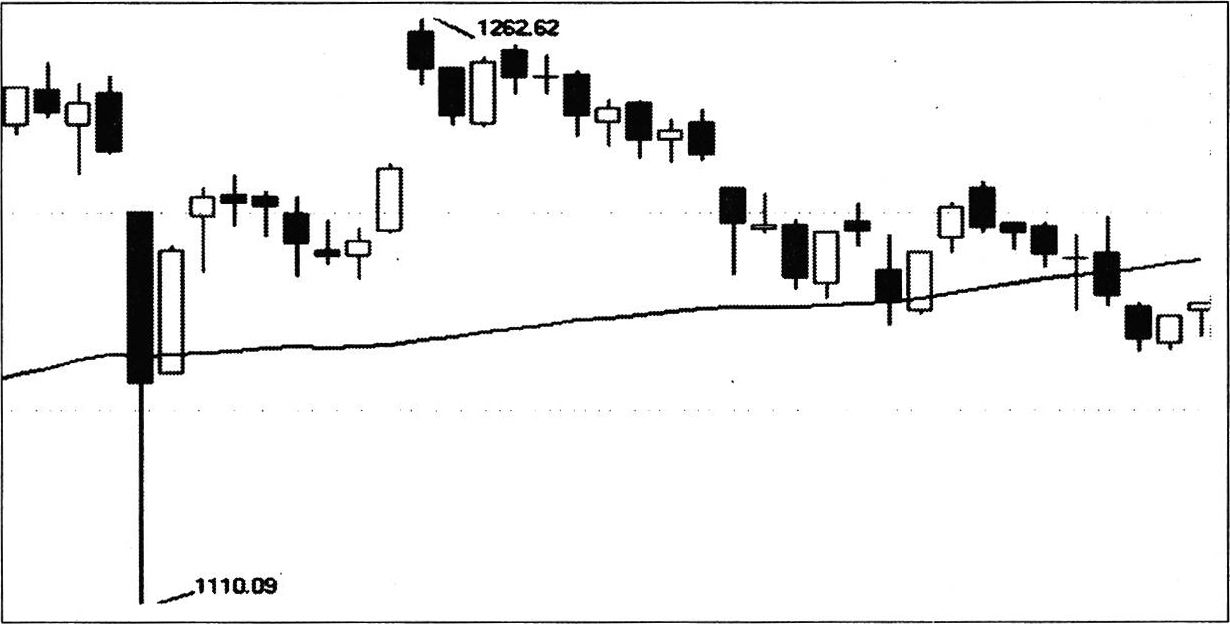
\includegraphics[width=0.88\linewidth]{images/4-11缺口形态示意图.jpg}
\caption{缺口形态示意图}\label{fig:gap-pattern}
\end{figure}

最后，缺口代表趋势强劲。几年前，山东神光提出一种不错的选股方法。只要周K线出现向上突破缺口，那么很可能出现强劲的上涨行情。在我来看，这种方法属于趋势思维，应该可以采纳。事实上，即使没有缺口，上涨就是买入最好的理由。

在我看来，缺口理论似乎更有理论研究的味道，分析行情可能会津津有味，但实战的价值不大。同样，单独的缺口理论也不可能构建起成环的交易系统。

\subsection{波浪理论}

{\kaishu
相对于波浪的“形”而言，我更加在乎的是波浪的“神”。或者说，相对于波浪理论的“精确”，我更加看重的是波浪理论的思想。

\hfill ——金融帝国
}

波浪理论继承了道氏理论中的很多宝贵思想，从而形成一种更精确的分析理论。道氏理论告诉我们何为大海，波浪理论告诉我们如何在大海中冲浪。波浪理论的起源来自于对道琼斯指数的研究，道氏理论的提出也是基于道琼斯指数。那么我或许可以用一部分道氏理论的思维方式来研究波浪理论。

首先，市场容量越大，波浪理论就越有效。有时我在想，波浪理论是否能够精确地适用于全部的市场品种呢？事实上，波浪理论同道氏理论一样，都是基于市场指数而产生的。如果将这种分析方法嫁接到个股上，那么效果就应该会大打折扣。我们不难发现，市场容量越大的品种，波浪理论的效果就越好。对于个股而言，大盘股的效果要好于小盘股。对于小盘股而言，并非波浪理论不起作用，而是这种作用更多地体现在波浪理论的思想，而不是波浪理论的精确。

其次，分析尺度越大，波浪理论就越有效。按照道氏理论的说法，长期趋势必然是由基本面的因素来决定的；中期趋势中人为因素只能干扰趋势；而短期趋势是完全可以人为操纵的。如果说波浪理论是一种市场特性的话，那么越是不容易人为干扰的尺度效果就应该越好。在行情低迷的2005年，你只要有几百万就能左右成交量稀疏的个股日内走势，也就是说，你的意志比波浪理论更容易对市场产生作用。

最后，股市比期货市场有效、比外汇市场更有效。毕竟波浪理论是起源于股市，其中包含了众多的股市特征。波浪理论考虑到股市随经济增长带来的涨跌不对称性。这或许就是，为什么上涨会是五浪，而下跌会是三浪的原因。对于外汇市场来说，直接标价法与间接标价法是完全对称的。人民币兑美元的走势，同美元兑人民币的走势是对称的。这样一来，波浪理论就失去了宏观上的有效性。

如果要想详细地介绍波浪理论，恐怕要照抄一本书了。这里我只是简单地把波浪理论分成几块来稍作探讨。

\textbf{黄金分割}

两个相邻的波浪之间通常会呈现黄金比例关系。有意思的是，从各个波浪的整体来看，他们通常也能符合黄金比例关系。黄金比例包括，0.236、0.382、0.5、0.618、0.764、1；以及他们的倒数，4.24、2.62、2、1.618、1.31。如果你将上证指数的中期波动，与相邻的中期波动作比例分析的话，你会发现它们经常会出现吻合。如果你能够将上证指数进行波浪划分，你会发现相同波浪的比例也可能是相同的。比如，二浪经常调整一浪幅度的100％和76.4％，而四浪调整三浪的38.2％、50％、61.8％等。

如果我们将上证指数1994年325点至2001年2245点持续七年的长期牛市进行波浪划分的话，你会发现一浪顶部位于0.382位、四浪底部也位于0.382位、三浪顶部位于0.618位；如果你将2001年2245点至2005年998点的长期熊市进行黄金分割的话，你也会发现A浪底部、B浪顶部也位于黄金分割位；同时长期熊市回调了长期牛市的61.8％。

\begin{figure}[htbp]
\centering
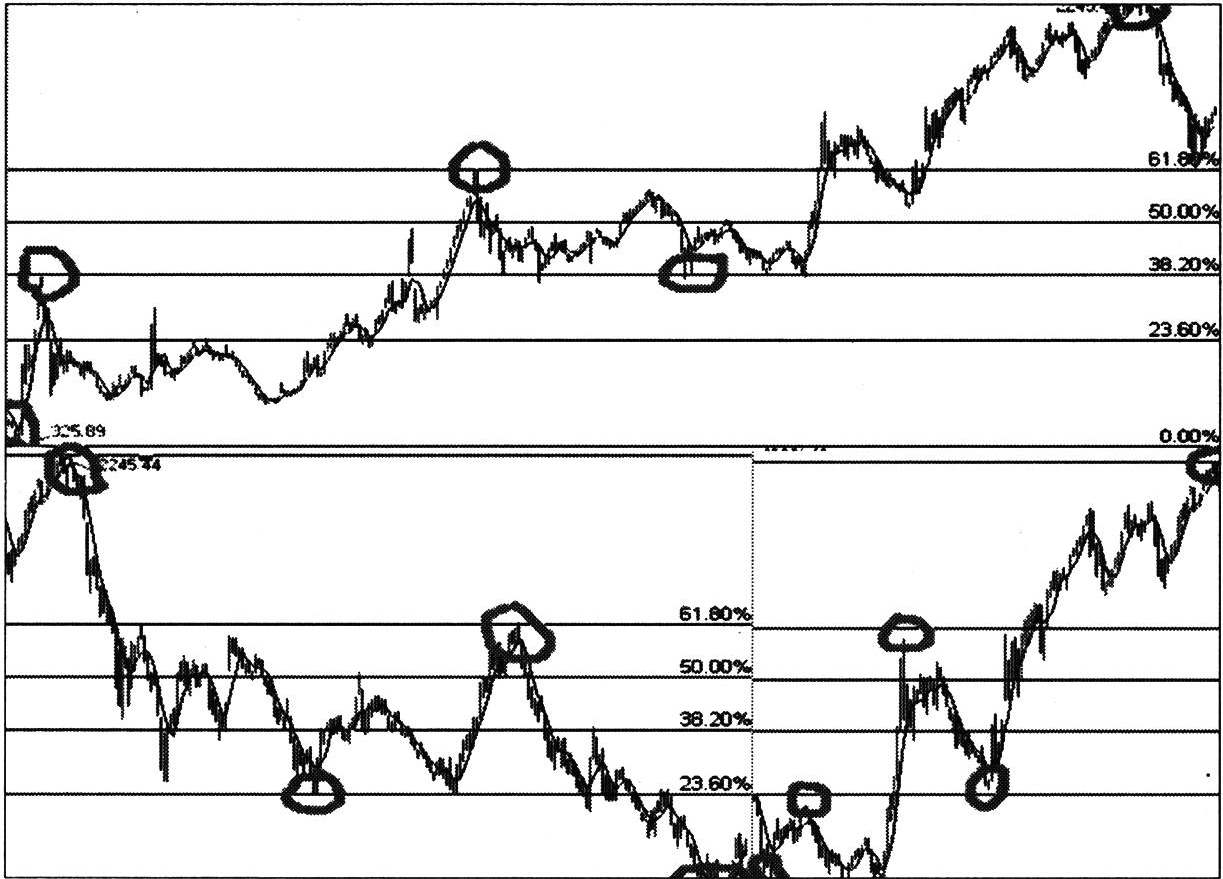
\includegraphics[width=0.88\linewidth]{images/4-12黄金分割与波浪比例示意图.jpg}
\caption{黄金分割与波浪比例示意图}\label{fig:fibonacci-wave}
\end{figure}

\textbf{平行线}

如果将二浪低点与四浪低点连接成一条趋势线的话，那么沿着三浪的高点就可以画出一条平行线。通常来说，五浪形成的最终顶部有可能就位于这条从三浪高点画出的平行线处。对于上证指数而言，如果将1996年初的513点同1999年的1047点连线，并以1997年1510点画出平行线，那么2001年的2245点正好位于此线处。

\begin{figure}[htbp]
\centering
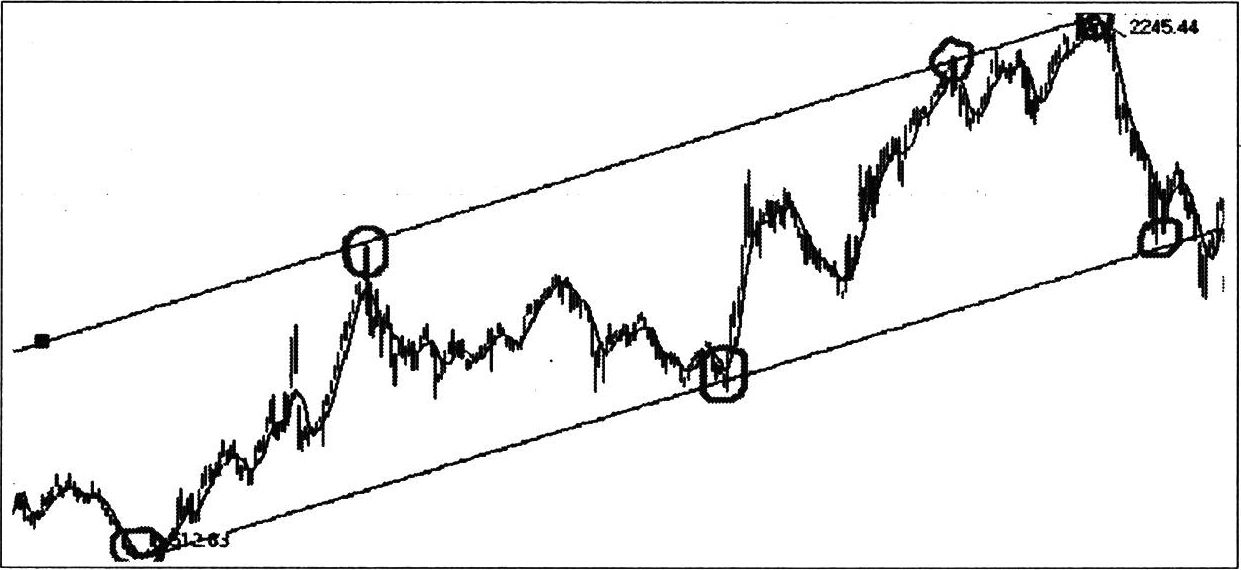
\includegraphics[width=0.88\linewidth]{images/4-13波浪平行线示意图.jpg}
\caption{波浪平行线示意图}\label{fig:wave-parallel-lines}
\end{figure}

\textbf{交替规则}

如果二浪调整简单的话，那么四浪调整就有可能复杂；如果二浪调整复杂的话，那么四浪调整就有可能简单。同时，如果三浪上扬简单的话，那么五浪上扬就有可能复杂（延长）；如果三浪上扬复杂（延长）的话，那么五浪上扬就有可能简单。我们可以发现，1996年的牛市运行德比较复杂，而1997年的牛市就运行得非常简单；同样1999年的牛市运行得非常简单，而2000年的牛市就运行得比较复杂。

\textbf{跌破四浪低点后见底}

按照波浪理论的说法：调整波尤其是第四调整波，其最大调整的结束位置是前一个次级的第四波调整的结束位置。从对上证指数的研究中，我们也能发现这种有意思的现象：调整波经常在略微突破前一个次级的四浪调整终点的位置结束，而我将这种现象称之为“四浪法则”。2001年以后从2245点至998点的调整可以清晰地划分成A、B、C三浪。而A浪结束的位置在1339点，这个点位正好跌破1999年底的1341点；而C浪结束的位置在998点，同样也是正好跌破1998年的1043点。其中1341点为1043点至2245点牛市的四浪回调低点；而1043点为325点至2245点长期牛市的四浪回调低点。

有时大B浪反弹，也会在大A浪第四子浪高点处结束。上证指数2001年底走出了大A浪下跌中的第四子浪反弹，最终结束于1776点。其后的大B浪反弹比较复杂，走出了平坦形的特征，最终B浪结束于2004年的1783点。

说实话，我最害怕别人问我为什么。曾经在与一位网友讨论“四浪法则”时，他一边感叹这种规律的美妙，一边还是忍不住地问我是什么原因产生了这种现象？这是我从来都没有想过的问题，正是这位朋友的可爱让我有了一些新的发现。或许这种现象，有可能产生于道氏理论的“权威的泥潭效应”。

按照道氏理论的说法，所谓牛市就是顶部与底部都不断抬高的行情，后面的底部要高于前面的底部。如果后面的底部低于前面的底部，那么就形成了一个牛市完结的信号。大家想想看，四浪的底部是否就应该是，大牛市见顶之前最后一个阶段性底部呢？也就是说，四浪底部被跌破时，才能够宣告牛市的完结呢？事实上，我们经常可以在市场上看到，对长期趋势的最后一波进行100％调整的中期牛熊市。当然，1997点5月至1999年5月的熊市，并没有调整至此前四浪底部之下。也就是说，上证指数没有调整到1996年底，《人民日报》社论所形成的855点之下。但有意思的是，如果我们打开深成指的走势图，519行情正巧是在股指跌破《人民日报》社论形成的低点之后发动的。关于“四浪法则”的案例，在本书最后的“网络文集”的“反弹宣言”中有更加详细的阐述，这里就不再重复了。

所谓“权威的泥潭效应”是指：当大众将某种权威的交易理论视为约定俗成的“公理”时，那么运用这种交易理论的效果就会大大降低，甚至还可能形成一种反向理论。比如说，海龟所使用的“唐奇安趋势”技术，因为海龟交易法则的披露，而使得该方法的收益率出现大幅衰竭的特征。或许这种方法已经成了趋势跟踪技术的最劣选择。甚至，因为形态理论早已深入人心，反过来使用该理论就比直接使用具有更大的价值。从前面的“点球原理”中大家不难发现：我的趋势跟踪技术完全基于均线系统，而并非是采用突破箱体的技术。我始终觉得，对于突破箱体而言，突破的提示意义过于明显，甚至更容易被大众集体接受，那么“突破”就有可能被用来刻意制造假信号。相反，均线系统的参数选择完全是个性化的，而绝对不可能形成某种典型性的假信号。事实上，超过半数的突破都有可能最终演化为假突破，而获利只能够更多地依赖于大赔率了。这时就出现了一种似乎可行的整理思路交易策略：当突破箱体或者创出阶段新高时，立即入场做空，同时设置一个紧密的止损点。

\begin{figure}[htbp]
\centering
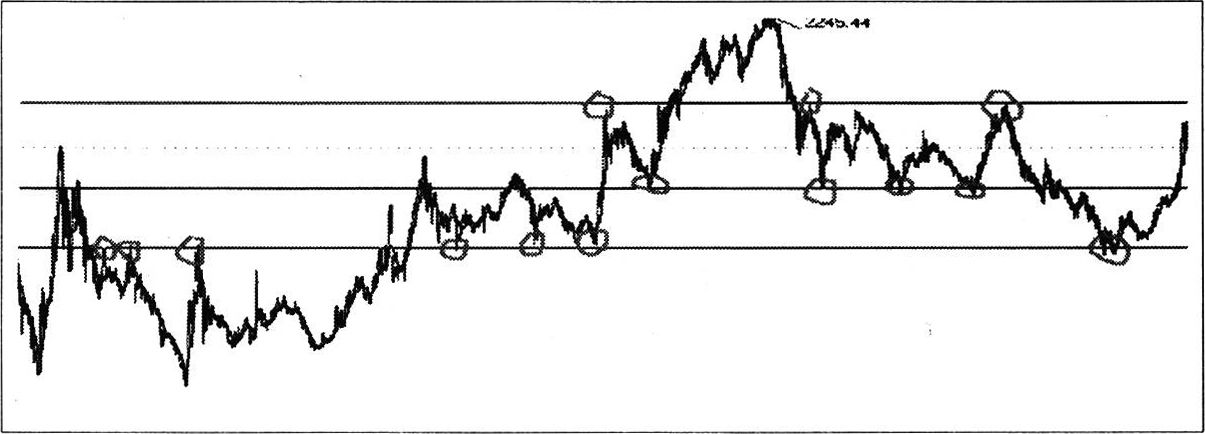
\includegraphics[width=0.88\linewidth]{images/4-14波浪交替规则示意图.jpg}
\caption{波浪交替规则示意图}\label{fig:wave-alternation}
\end{figure}

如果我们再仔细地研究各波浪内部结构的话，我们就能发现后面提到的“股市层次理论”；如果我们再仔细研究波浪形态的话，那么就能发现形态理论中的不足，从而找到后面提到的“反形态理论”。

我在回顾历史行情的时候，总能感到一种波浪理论带来的奇妙感觉。但我并不否认，这种感觉的确很少在事先出现。这里点到为止地阐述一些波浪理论的常识，感兴趣的朋友可以找一些波浪理论的书籍来阅读。不过我还是希望读者朋友不要陷入微观上“数浪”的怪圈，多了解一些波浪理论的思想也许会有更好的效果。

事实上，波浪理论恐怕是大家争议最大的理论。甚至很多交易大师，也都认为该理论完全是主观的故弄玄虚。那么，我会如何看待波浪理论的价值呢？波浪理论真的是毫无用处吗？在我看来，一种市场理论是否有价值，并不一定要求它拥有预知未来的水晶球。K线图是否有价值呢？无论是赢家还是输家都是在看相同的K线图，因此交易者是否能够盈利并非取决于所使用技术的本身。在我看来，波浪理论同K线图一样，都是一种出色的对于市场高度概括下的表述方式。很显然，波浪理论能够使我们拥有一种简洁的思维方式。

波浪理论是否有用的答案，完全取决于你需要用波浪理论来干些什么。如果你想找到能够预知未来的水晶球，那么波浪理论显然难以胜任。在我看来，波浪理论最大的价值就在于对行情进行阶段分类，从而寻找市场在不同阶段所表现出的特性。这就好像我们可以把人通过年龄阶段归类为儿童、青年、中年、老人，即使我知道你是一位青年人，但是我也无法回答你买彩票是否会中奖的问题。很显然，这种归纳只能够给我们关于某些问题概率上的提示，而绝对不可能回答出任何确切的答案。我们只能够说年轻人通常比老年人更加健康，但无论如何也无法在个体上绝对肯定这一点。我们可以对历史上壮观的大牛市进行阶段性研究，并且发现一些具有共性的规律。比如说，一波疯狂的投机狂潮往往都会经历这样的阶段：市场先上涨到一个让大众咋舌的高价，从而参与者都认为这种不理智的投机行为使得价格太贵了。而第二个阶段更加有意思，市场终于上涨到了更高的价位，但市场参与者反而找到了高价的合理性，甚至认为买入是一种安全的投资。事实上，大众集体推崇价值投资往往需要两个条件：第一，价格经过大幅上涨，从而形成明显的获利效应。第二，相当一部分市场参与者已经出现了小幅亏损。其实，我之所以反感价值投资，很大一部分原因是因为大众总是拿它当做逃避亏损的借口，而在获利时进行长期投资简直比登天还难。在后面的“雕虫小技”中，大家可以看到“股市层次理论”，这是一种更加个性化的阶段性分析。虽然我们不能回答出市场未来会如何运行，但我们却可以使用排除法来回答市场不太可能的运行方式。比方说，股市中所有的股票都一致性上涨，往往不太可能直接形成最终的牛市顶部。

另一方面，波浪理论虽然无法预测未来的走势，但却可以帮我们寻找价格不太可能稳定的市场阶段。当你看到一个标准的头肩顶后，你会想些什么呢？很显然，无论是认为股价会大幅上涨，还是认为股价会大幅下跌都是非常荒唐的事情。毫不夸张地说，这种形态对于涨跌没有任何提示作用！即使是这样，我也能够知道自己将要大赚一笔了！道理很简单，无论是头肩顶后的暴跌，还是“跨过顶部是天空”后的暴涨，总之，市场出现壮观的趋势行情概率极大。那么我所使用的连续不间断趋势跟踪系统，将会在短期内赚取不小的利润。对于连续不间断趋势跟踪系统来说，重要的并非是判断市场未来的涨跌，而是寻找适合作为跟踪开端的“赌点”。由此可见，如果用弹性的、概率式的思维方式来使用波浪理论，那么波浪理论的确存在美妙的价值。反之，用刚性的、预测式的思维方式来运用任何市场理论，恐怕都是没有丝毫价值的。

对于我来说，相对于波浪的“形”而言，我更加看重波浪的“神”。要知道，我在数浪的过程中绝对不是非常严谨的，甚至可能是非常模糊的。这里我可以举两个例子。第一个例子是，从2001年2245点至1339点的大A浪下跌中，我将1515点至1776点的之字型调整定义为小四浪。如果有人问我小二浪在哪里？那么我一定回答不知道！对于我来说，那次反弹具有明显的四浪特征，并且此前的下跌具有明显的主跌浪特征就已经足够了。第二个例子是，我对从1994年325点至2001年2245点长达7年的长期牛市的子浪进行划分时：将1994年的1053点定义为一浪的高点，而将1998年的1043点定义为四浪的低点。显然这与波浪理论的规则有矛盾之处，但我并不会纠结这些细枝末节。或许有人会问，我对波浪的画法对吗？我觉得问这种问题的人，一定是并不了解波浪理论真谛的人！我始终相信，波浪的画法并没有绝对的正确答案，而只要是适合自己（角度）的阶段划分即可。或者说，这种阶段归纳方式有助于我对市场的理解即可。很显然，具有唯一正确答案的理论，一定无法描述真实世界的发展！这就好像，我们可以将人归纳为儿童、青年、中年、老年；也可以将人归纳为白种人、黄种人、黑人。至于该如何归纳，完全取决于我们要回答什么样的问题，而归纳的方法绝对不可能是唯一的。

\subsection{江恩理论}

{\kaishu
在应对无参数的市场时，我采用的是有参数的趋势跟踪系统。我很肯定这并非最好的方法，也许最好的方法是设计出基于“形态”与“时空关系”而建立的无参数系统。

\hfill ——金融帝国
}

江恩的理论体系从根本上说就是在看似无序的市场中建立严格的交易秩序。请注意，是交易秩序而不是行情预测。江恩理论的技术分析方法，把价格与时间巧妙地加以结合乃是独一无二的。下面我就粗略地谈一下我眼中的江恩理论。

\textbf{时间换空间}

历史上，我们可以清晰地发现从横向整理的时间换取大幅波动空间的案例。2001年上证指数快速从2245点下跌至1339点，如此快速的下跌速度让很多老股民都大跌眼镜。有意思的是，如果我们将2000年8月22日的2115点与2001年2月22日的1894点连接画一条X线，那么上证指数两次跌破这条X线后都走出了大幅反弹的行情。这是否说明，2001年的快速下跌，和此前将近一年的横向整理有某些相关性呢？无独有偶，1998年8月上涨指数同样走出了快速暴跌行情，那是一次从缓慢下跌演化而成的快速下跌。如果我们将1998点6月16日的低点画一条下降江恩线1×1角度线的话，那么这条线同样扭转了快速下跌的颓势。

\textbf{熊市生命线}

如果我们对历史行情进行统计的话，那么就不难发现很多中期熊市的下跌速率都是相同的。很多初学者都认为江恩线不容易绘制，毕竟行情软件中“时空”比例是不同的。这也是曾经困扰我的一个难题，最后的解决办法就是：找出一条由典型行情绘制出的趋势线，假设其为1×1角度线，然后按照倍数关系绘制其他的角度线。

这时我们可以发现，从显著顶部画出的江恩下降2×1角度线就成为熊市的生命线，当价格涨过该线后，熊市就结束了。有意思的是，在过去十年的时间内，这条熊市生命线的角度从来都没有改变过。下图中的全部画线都是平行线，而绝对没有进行任何优化。

\begin{figure}[htbp]
\centering
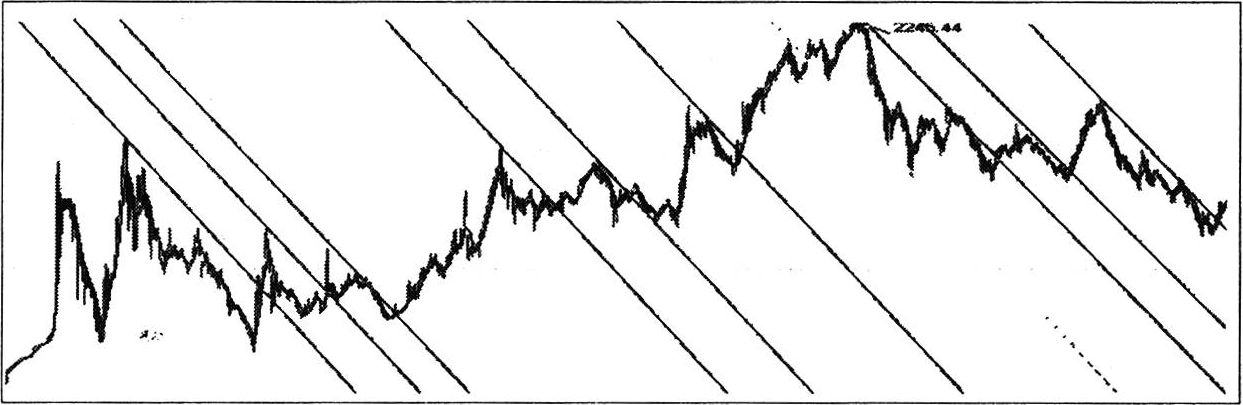
\includegraphics[width=0.88\linewidth]{images/4-15江恩下降角度线示意图.jpg}
\caption{江恩下降角度线示意图}\label{fig:gann-down-angle}
\end{figure}

\textbf{定速线}

如果我们将中期牛熊波动的高低点连线，也会发现这些线通常也是平行的，他们通常是江恩1×1角度线。同时我们还会发现一个更有意思的现象：通常中期熊市的前半段会沿着这条定速线（也就是压力线）下跌，其后会横向盘整出这条定速线，最后行情又会非常迅速地“砸”向这条定速线。熊市结束前的最后一“踹”，通常都是快速而恐怖的。这不由让我感到，快速下跌是由此前横向整理的时间所换取的！上面提到的1998年8月的暴跌，也是由起初缓慢的下跌而换取的。这又不由让我感觉到，市场居然像公交车一样准时！公交车到达终点站的时间都是固定的，如果司机前半段由于某种原因而开得非常缓慢，那么后面的路程就必须用非常快的速度来赶时间。

\begin{figure}[htbp]
\centering
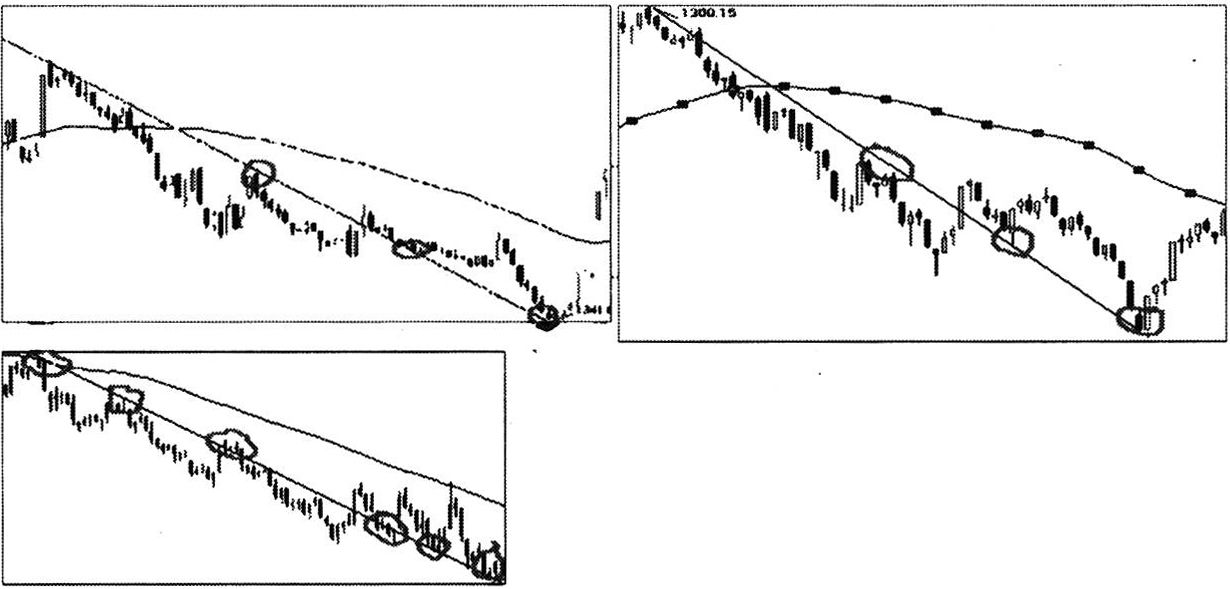
\includegraphics[width=0.88\linewidth]{images/4-16江恩定速线示意图.jpg}
\caption{江恩定速线示意图}\label{fig:gann-fixed-speed}
\end{figure}

\textbf{时间周期}

这恐怕是最难让交易者理解的部分了，当然我也无法理解所谓的时间周期。曾经我发现1997年、1998年、1999年的高点都是精确地间隔13个月。1997年5月至1999年5月的调整历时2年零半个月，而1999年5月至2001年6月的上涨也历时2年零半个月……

在我看来，江恩理论也许能够将时间与空间融合，而得出并不固定的多个解，从而创造完美还是说得通的。但我绝对不相信，江恩理论能够将价格与时间分离而进行单独预测！我提醒交易者不要陷入时间周期的怪圈中。要知道，时间周期即使用“事后合理”的方法，也很难找到完美。我曾经听说一位分析师，是在一边数日子、一边套用时间周期来给交易者“讲课”的。我真的不懂时间周期，但我相信使用时间周期的那些所谓的大师们，也未必就一定真的明白时间周期。

几年前我看到一本《江恩投资实战技法》的书籍，并由此开始了幻想。书中总结了江恩线的使用规则，而我用这些规则套用在上证指数的历史行情时，发现真的是太完美了！我本想在本节中引用这些规则，然后再从上证指数中找出实例。但在我还没有弄清这些完美的本质之前，并不想给大家过多的误导。我很肯定这其中存在事后合理的偏向，但我又无法得知其中具有的真实价值到底有多少。

在应对无参数的市场时，我采用的是有参数的趋势跟踪系统。我很肯定这并非最好的方法，也许最好的方法是设计出基于“形态”与“时空关系”而建立的无参数系统。在我看来，使用系统获利的关键并不在于系统的优劣，而是在于使用者的心灵境界。有时我真的感慨，交易利润完全是来自于对心灵折磨的补偿。我相信这种无参数的交易系统，绝对比趋势跟踪系统需要更高的心灵要求。要知道，我在进行趋势跟踪时，也仍旧会经常出现心理问题。我相信，在没有达到心灵的绝对成熟以前，过多的想入非非只会让我们走火入魔。达芬奇的成长离不开长期“画鸡蛋”的过程，那么交易者的成长似乎也仍旧无法摆脱长期通过规则来约束本能的过程。无论是随心所欲的创作，还是随心所欲的交易，恐怕都是初学者所望尘莫及的。

\clearpage
